\begin{fig}{\linewidth}\unskip
  \newcommand{\greytitle}[1]{\centering\footnotesize{\color{black!40!white}#1}\bigskip\par}
  \begin{minipage}[t]{0.30\linewidth}
    \greytitle{Northern Ontario}
    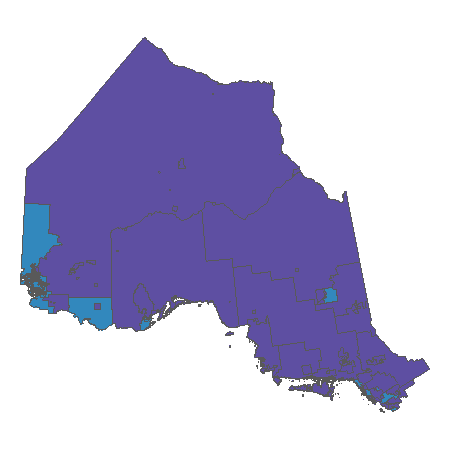
\includegraphics[width=\linewidth]{ontario-north}
  \end{minipage}\hfill%
  \begin{minipage}[t]{0.32\linewidth}
    \greytitle{Southern Ontario}
    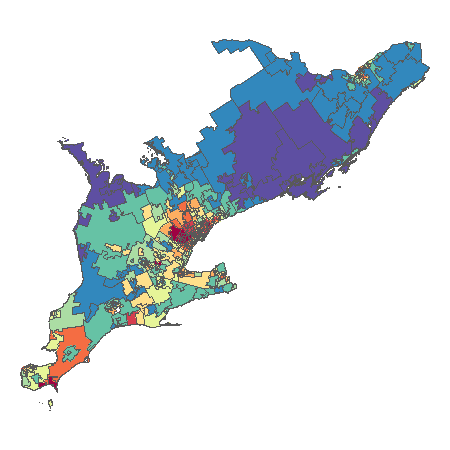
\includegraphics[width=\linewidth]{ontario-south}
  \end{minipage}%
  \begin{minipage}[t]{0.36\linewidth}
    \greytitle{Greater Toronto Area}
    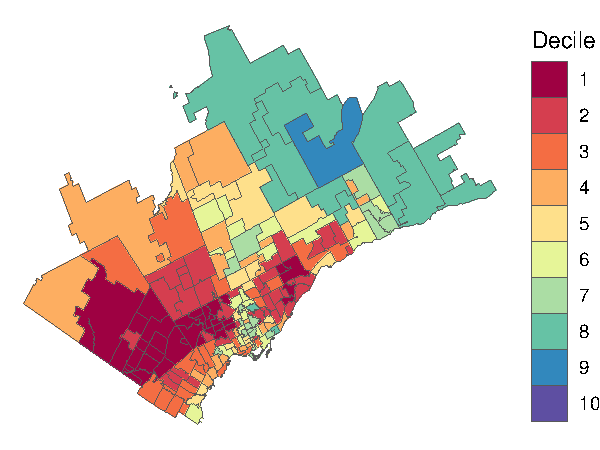
\includegraphics[width=\linewidth]{ontario-gta}
  \end{minipage}
  \caption{Map of 513 Ontario areas grouped into 10 patches (deciles)
    by \textsc{covid-19} incidence}
  \label{fig:ontario}
\end{fig}
\medskip\par
\paragraph{Notation:}
\begin{tabular}[t]{llllll}
  $g$~: & self patch  & $a$:  & self age group  & $y$: & contact type \\
  $g'$: & other patch & $a'$: & other age group &      &
\end{tabular}
\paragraph{Main Output:} $C_{gag'a'y}$: \# daily contacts of type-$y$ per-person formed
\par\indent from patch/age $ga$ to patch/age $g'a'$
\paragraph{Context:}
513 Ontario areas grouped into 10 patches by \textsc{covid-19}
\par\indent incidence (Figure~\ref{fig:ontario}) \& population stratified into 5-year age groups
\paragraph{Data:}
\begin{itemize}
  \item Population distribution by age and patch $P_{ga}$ $\leftarrow$ Census \cite{StatsCan2016} (Figure~\ref{fig:Pga})
  \item Mobility matrix $B_{gg'}$ $\leftarrow$ Cell phone data \cite{Ghasemi2021}\par
  \% residents who travelled from $g$ to $g'$ daily, including within-patch \&\par
  \% reduced mobility during $t$ = April 2020 vs Jan--Feb 2020 (\textsc{ref})
  \item Age contact patterns $C_{aa'y}$ $\leftarrow$ \citet{Prem2021}\par
  \# daily type-$y$ contacts per-person from age group $a$ to $a'$
\end{itemize}